\chapter{System evaluation} \label{ch:eval}
The evaluation of the system is used to determine the effectiveness of the natural language instruction-based control. The focus of this test is verbal flexibility. The system is built on sets of keywords used to connect words to actions. In itself, it would mean that words that do not appear in the database would not be usable. But since the system makes use of a cosine similarity comparison method, words outside the database should be interpretable. Another focus is the NLP pipeline in general, as this pipeline is most likely to introduce errors as it solves a complex task (NLP) compared to the information transformation task the parser and the kinematics pipeline do.
\\
To get natural language instructions, it is thought that the best approach is to use other humans as test users.
These people cannot know what the system is capable of and are therefore not biased toward using words that appear in the database. 

As the system was meant to be intuitive for the end user, it was evaluated on test users with no previous experience with the system. To avoid bias, the test users were not made aware of which words appeared in the database.
This chapter explains how the test is set up and the results obtained.

\section{Test setup}
The test is a series of three tasks that the test users must solve using the robot manipulator. The test users are given a video of the robot solving the task, which is used to show what the user must make the robot do. The video presentation is used because it introduces no wording bias, as the user is not given any words during the presentation. The test users write an instruction intended to be executed on the robot to copy the movements seen in the video. The three tasks are shown in the video linked below.\footnote{https://www.youtube.com/watch?v=zVLaS9Vfv1k}
Figure \ref{fig:task1}, \ref{fig:task2} and \ref{fig:task3} shows the step-by-step actions executed on the robot arm.

\begin{figure}[ht]
    \centering
    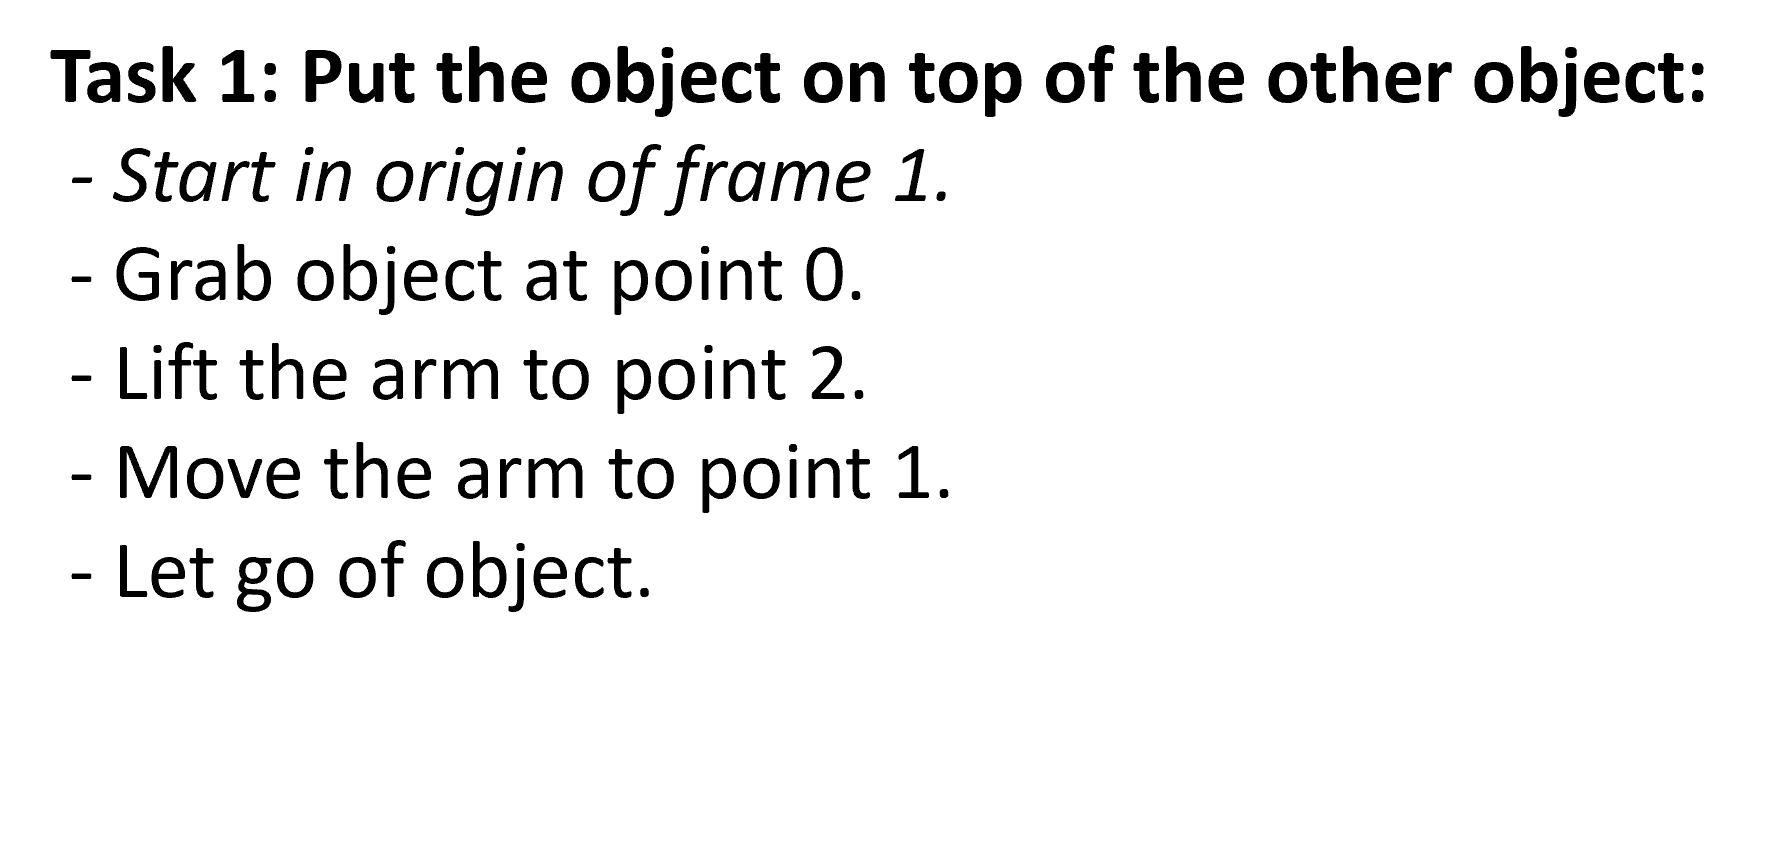
\includegraphics[width=9cm]{img/Task1.png}
    \caption{List of actions done in task1.}
    \label{fig:task1}
\end{figure} 

\begin{figure}[ht]
    \centering
    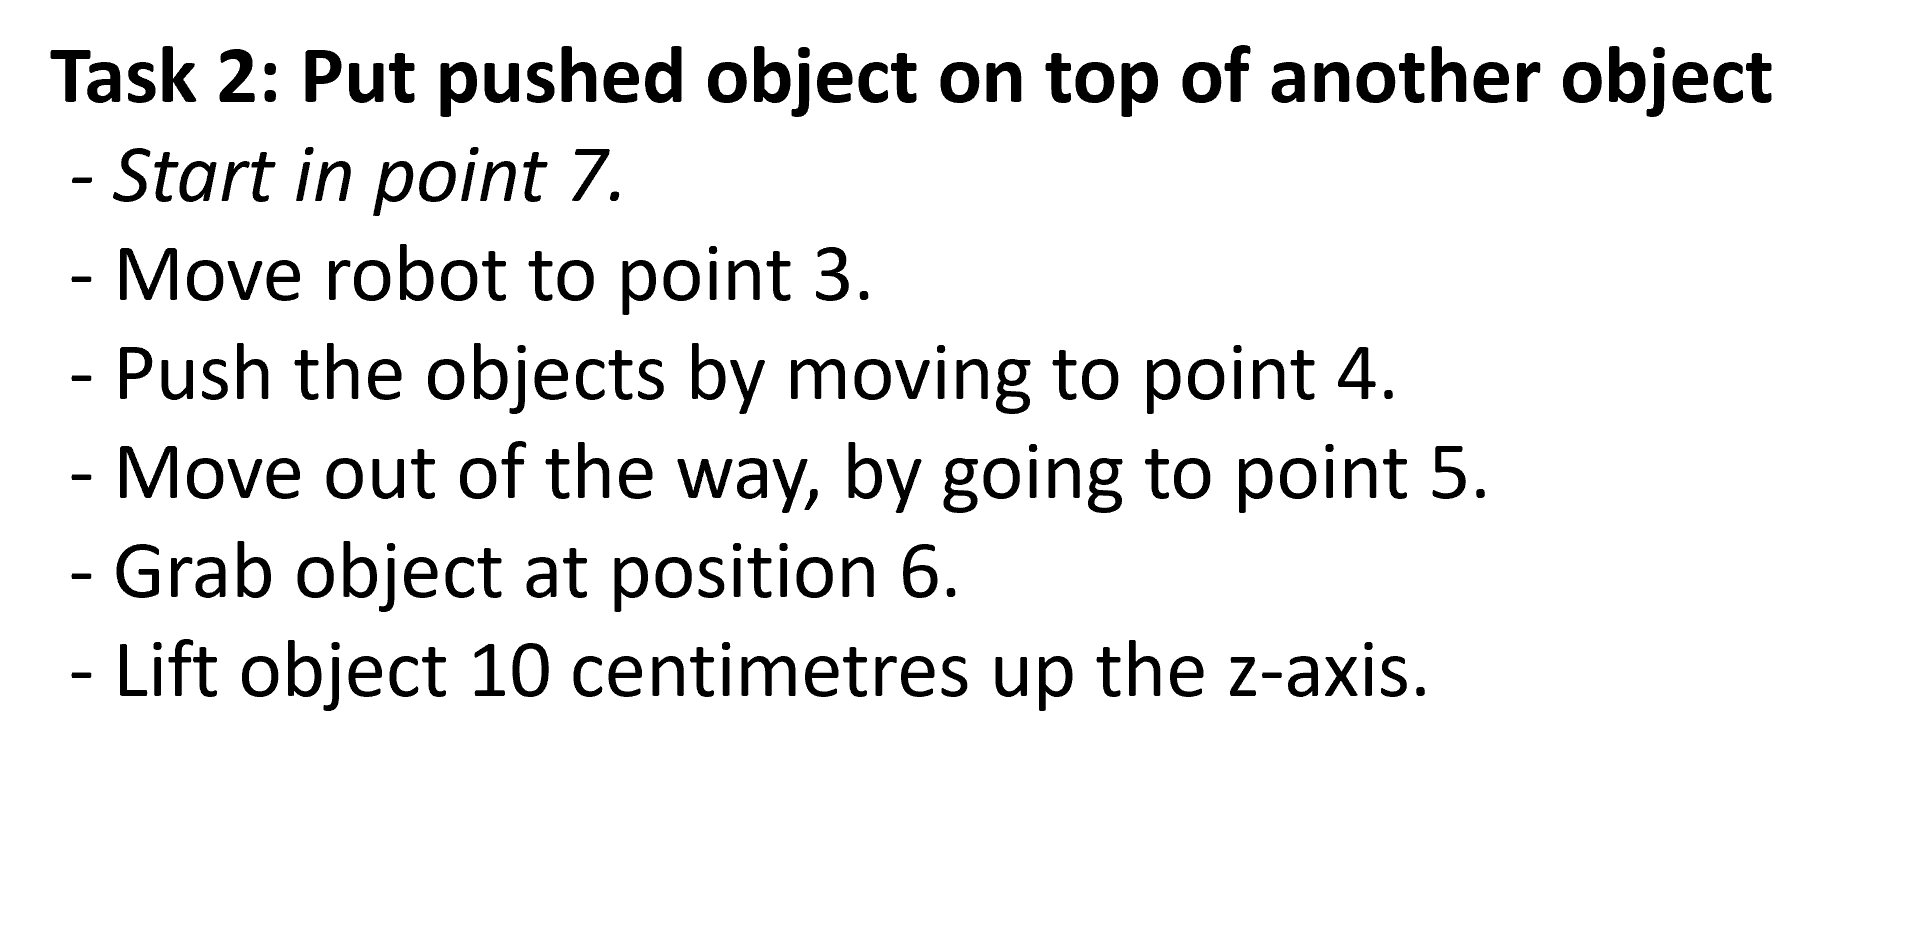
\includegraphics[width=9cm]{img/Task2.png}
    \caption{List of actions done in task2.}
    \label{fig:task2}
\end{figure} 

\begin{figure}[ht]
    \centering
    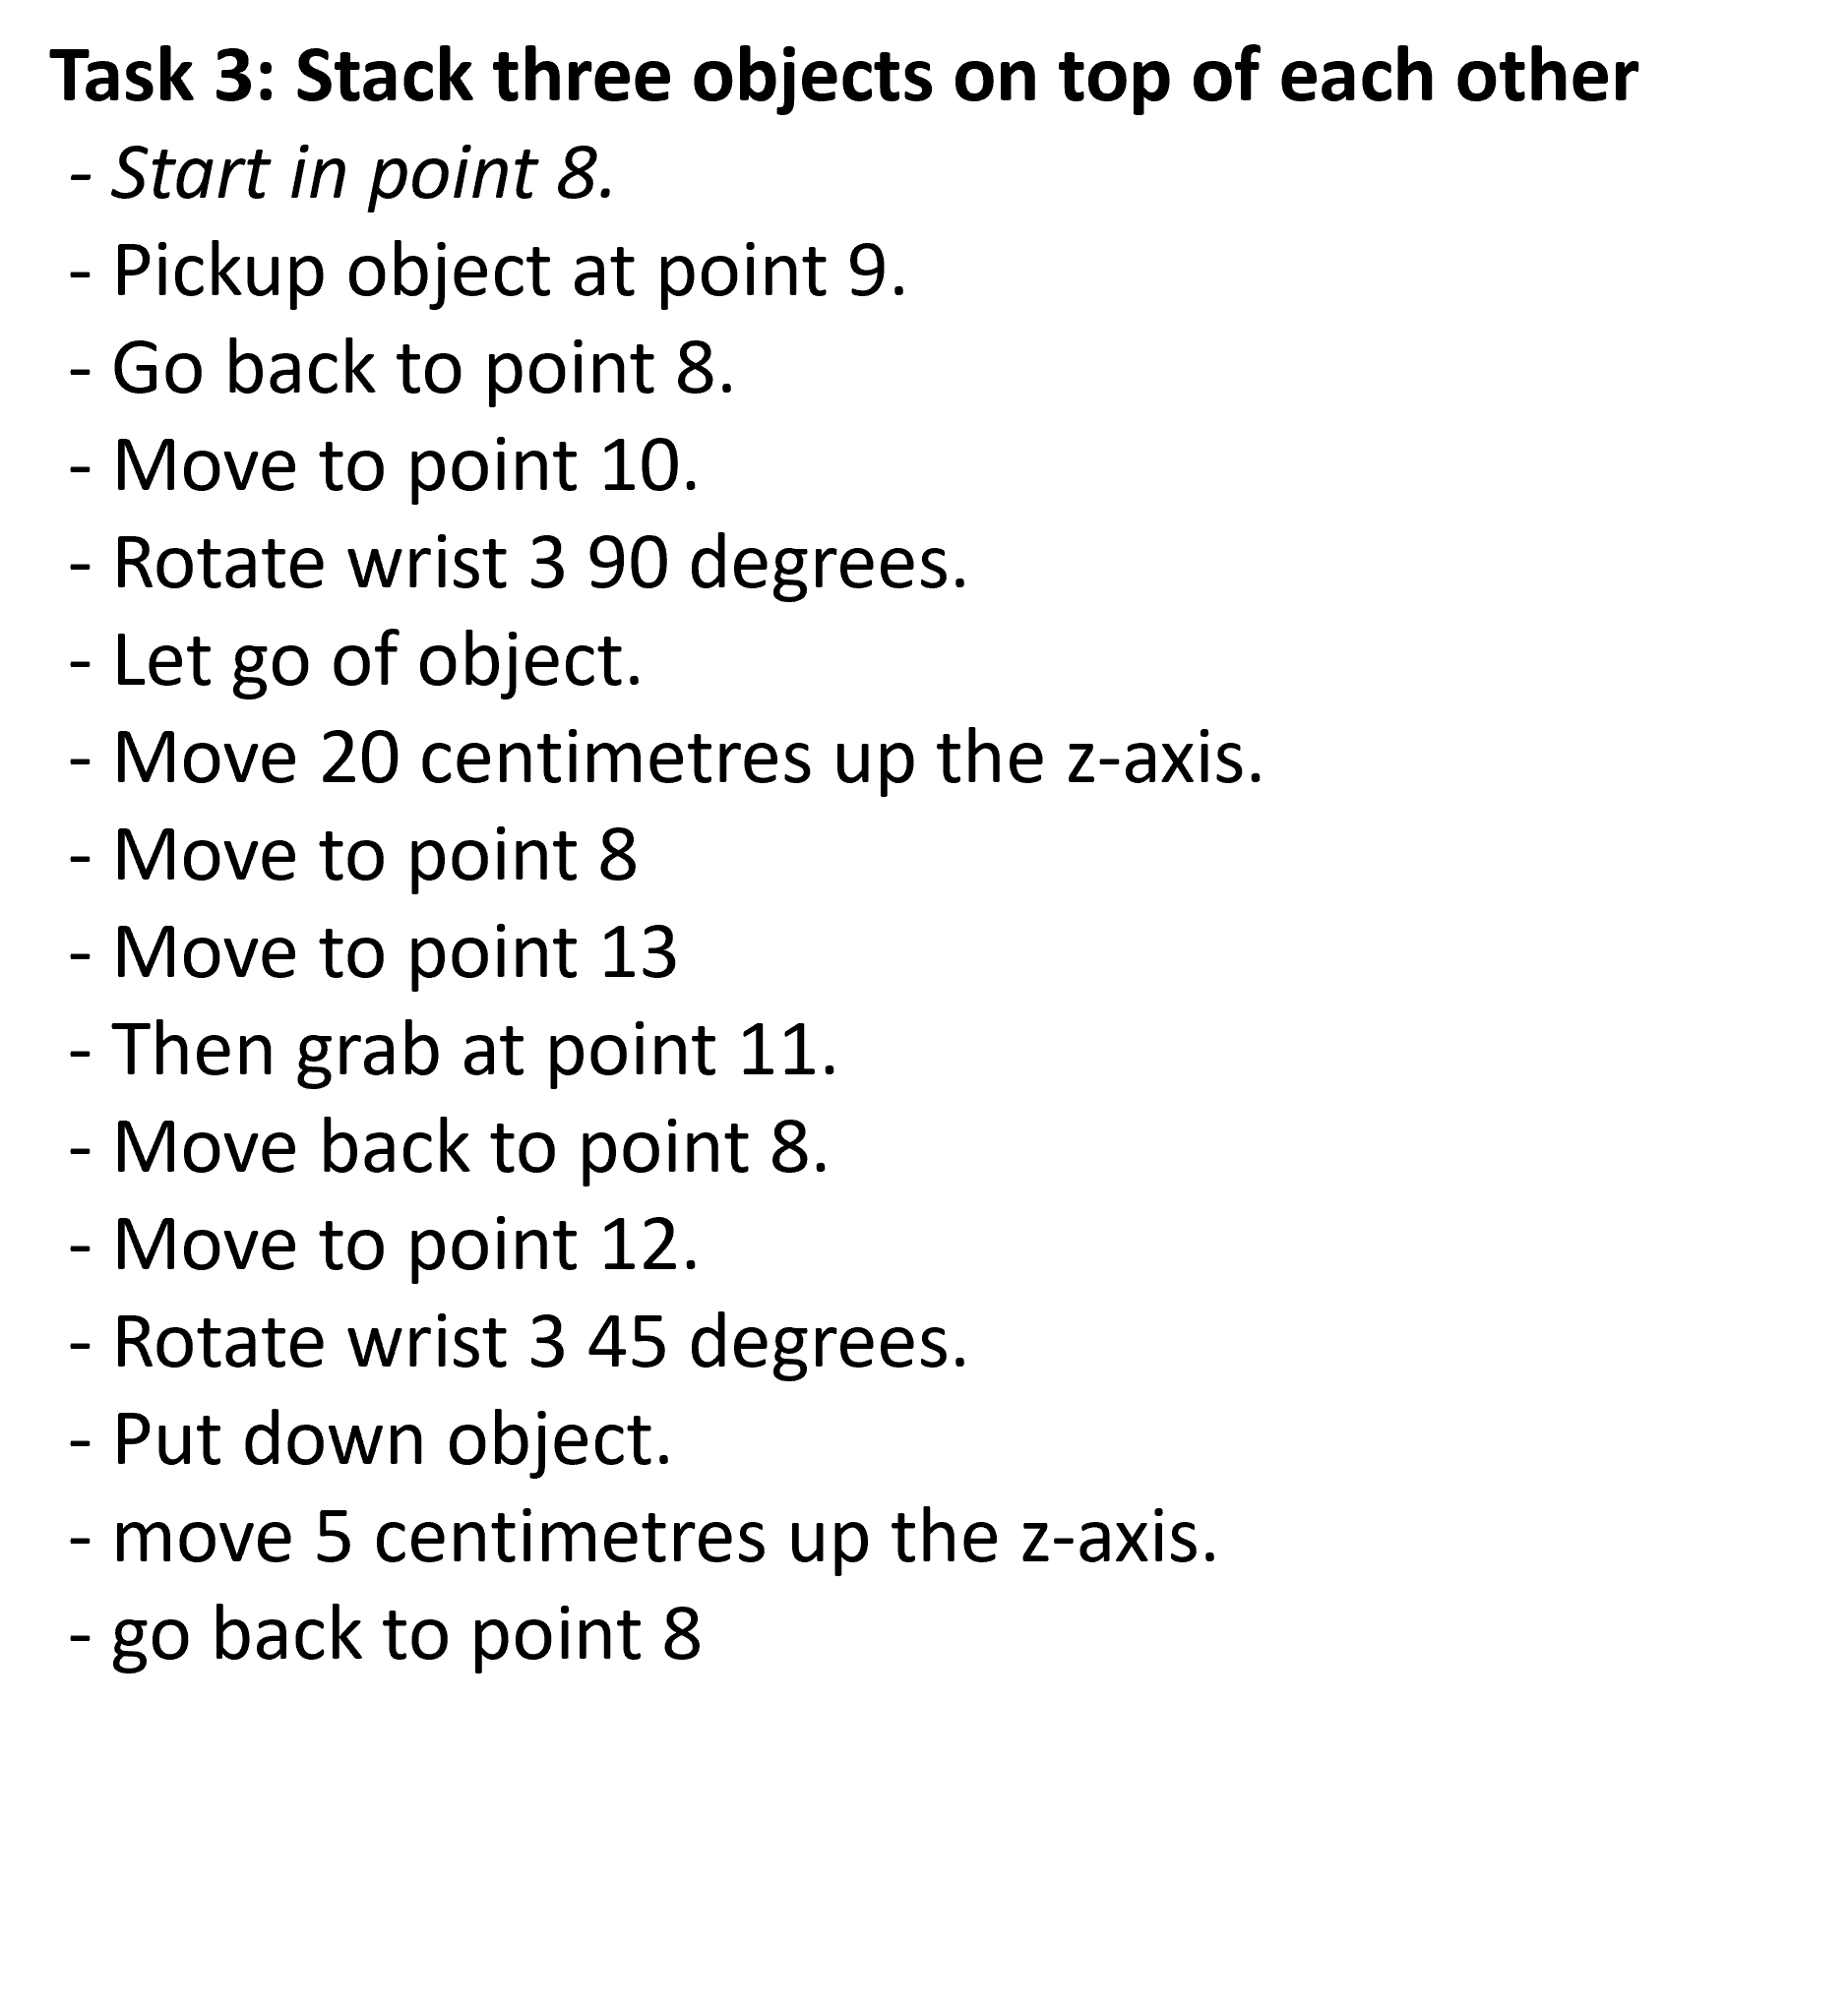
\includegraphics[width=9cm]{img/Task3.png}
    \caption{List of actions done in task3.}
    \label{fig:task3}
\end{figure} 
The videos present a robot manipulating 2 to 3 objects in its environment. The tasks are designed to heavily use the 'move' action, as it is the most important action the system has. It was deemed a lower priority to get tasks that made the user do the meta action 'repeat' or the system actions 'set point' or 'set frame'. Therefore, due to time constraints, no tasks were made that used the given actions.
\\
The instructions of the test users were collected and replayed on the system to test if the robot acted as intended.
\section{Test results}
Figures \ref{fig:eval_test_TOTAL}, \ref{fig:eval_test_1}, \ref{fig:eval_test_2} and \ref{fig:eval_test_3} present graphs that show the test results. Each task was solved by 10 people. All the actions combined from all three tasks sum up to 29 actions. This gives a total of 290 actions tested on the system. The first graph shows the success ratio of all the action types throughout the test. The next three graphs show the success ratio of all individual actions in the given task. The cosine similarity threshold was set to 0. But through further investigation, it was shown that the lowest needed threshold for this sample data was 0.40. The lower similarity score came from the instruction "Slide to point 4", where the instruction was first accepted when the system guessed the word "slide" as "move" with a score of 0.40.
Figure \ref{fig:error} shows the type of errors made, which will prove useful when discussing the nature of the errors and how to improve the system. Furthermore, figure \ref{fig:error_num} shows the number of errors produces, relative to successful commands.

\begin{figure}[ht]
    \centering
    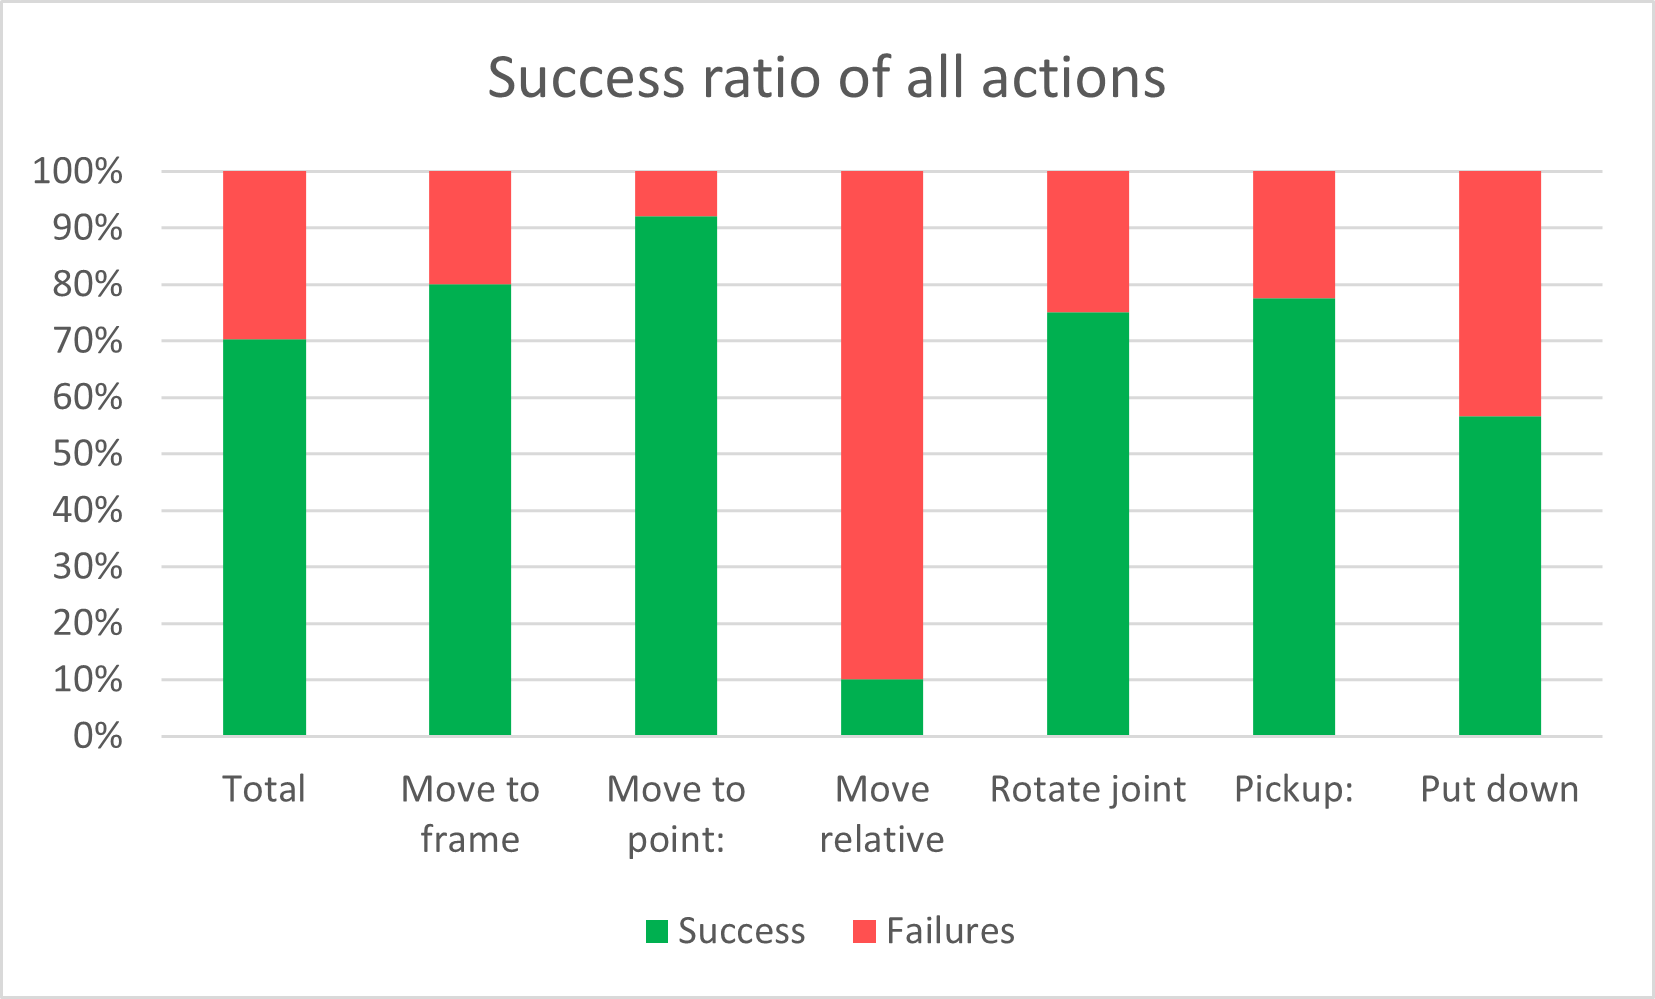
\includegraphics[width=9cm]{img/test_results_TOTAL.png}
    \caption{Graph illustrating the success ratio of all actions in the whole test.}
    \label{fig:eval_test_TOTAL}
\end{figure}



\begin{figure}[ht]
    \centering
    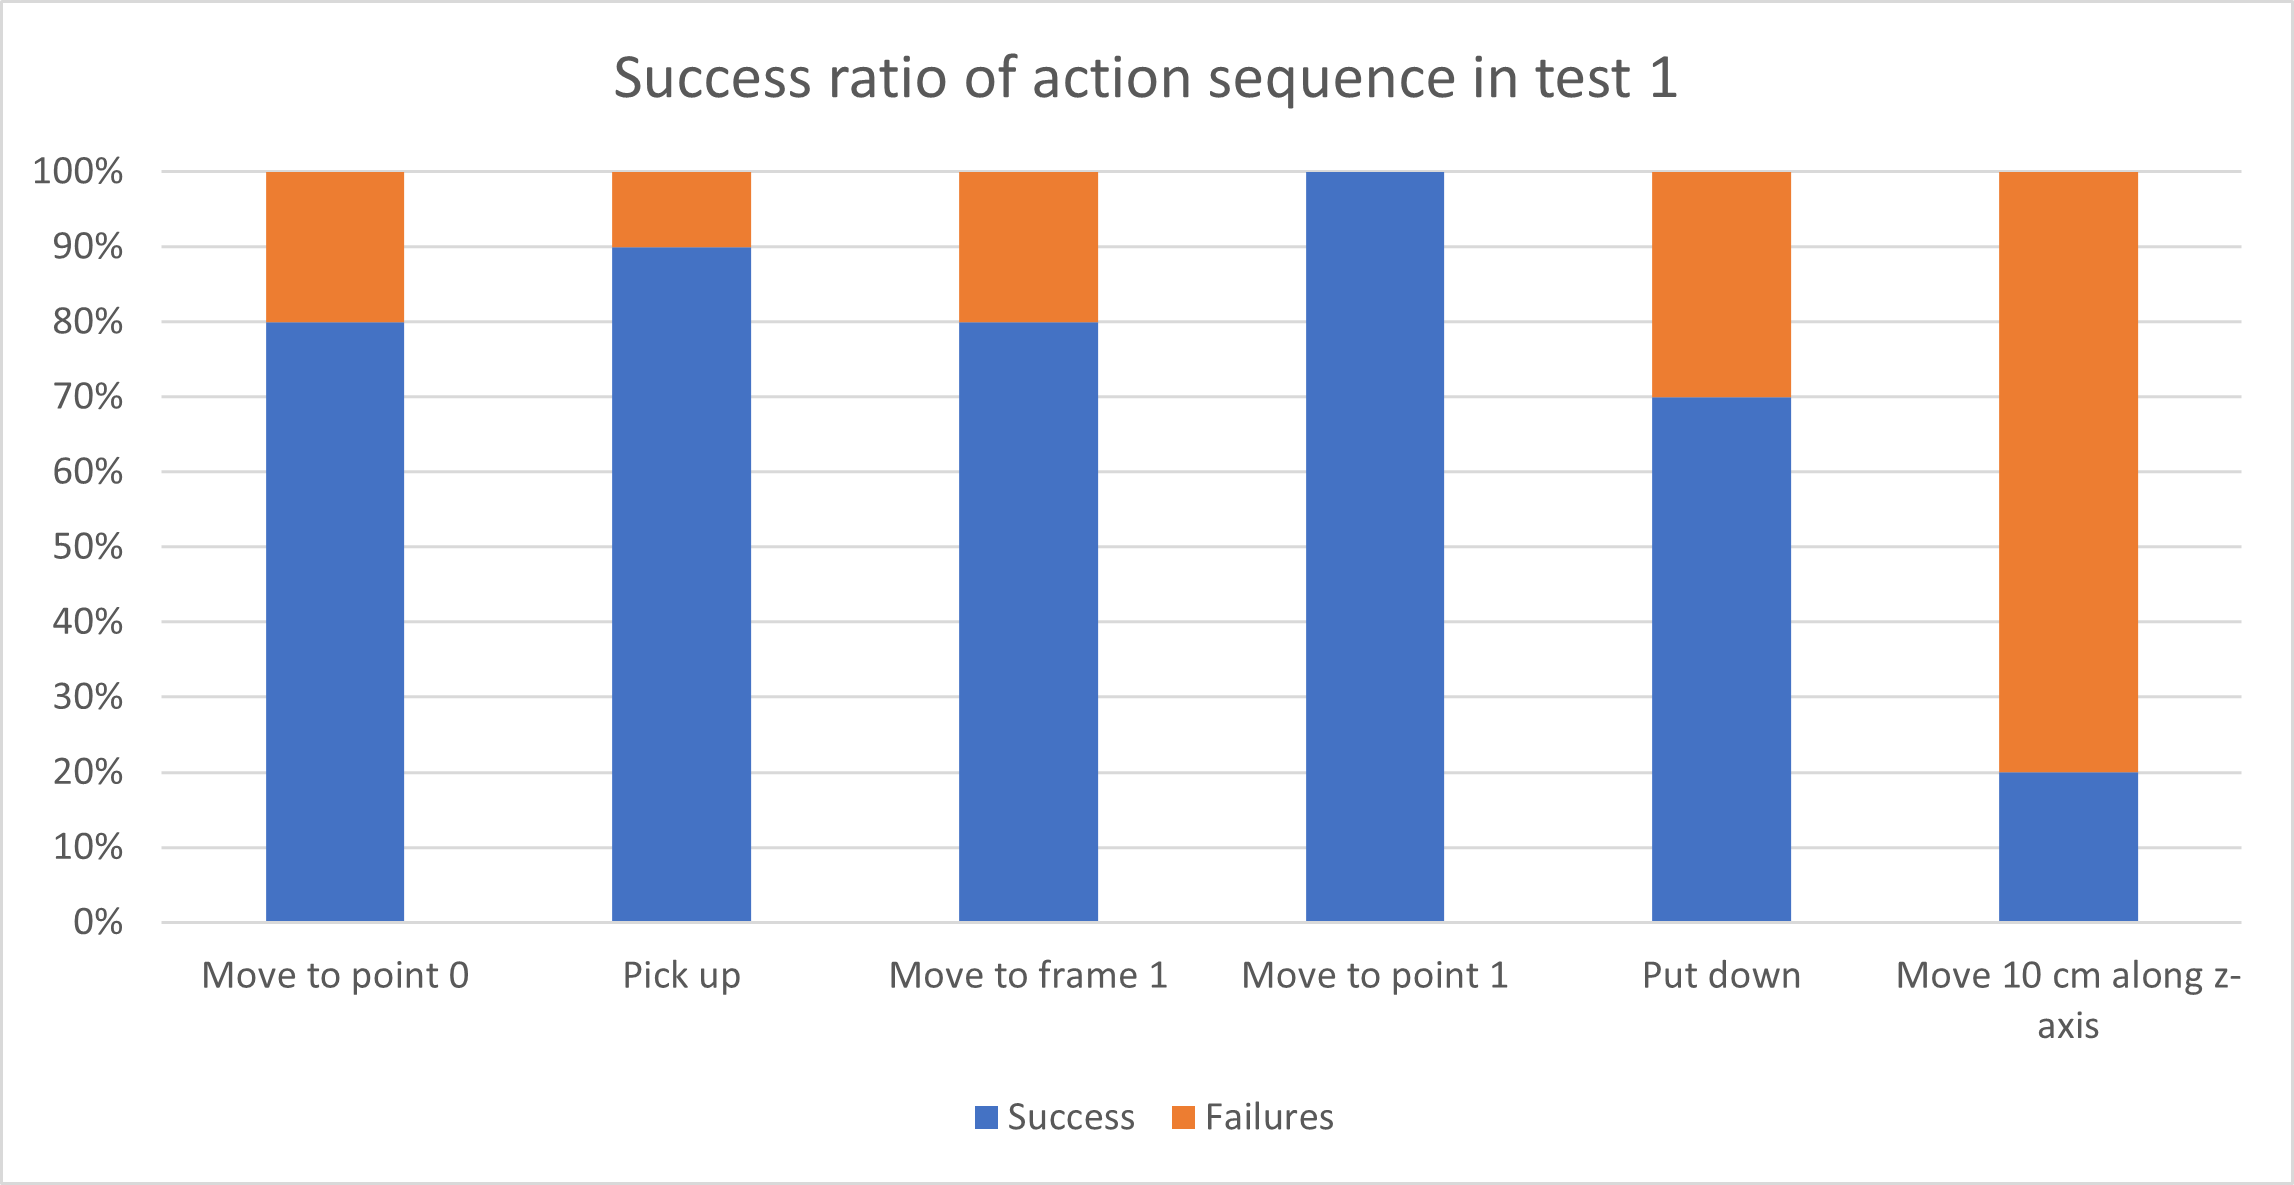
\includegraphics[width=9cm]{img/test_results_1.png}
    \caption{success ratio of each action in task 1.}
    \label{fig:eval_test_1}
\end{figure}

\begin{figure}[ht]
    \centering
    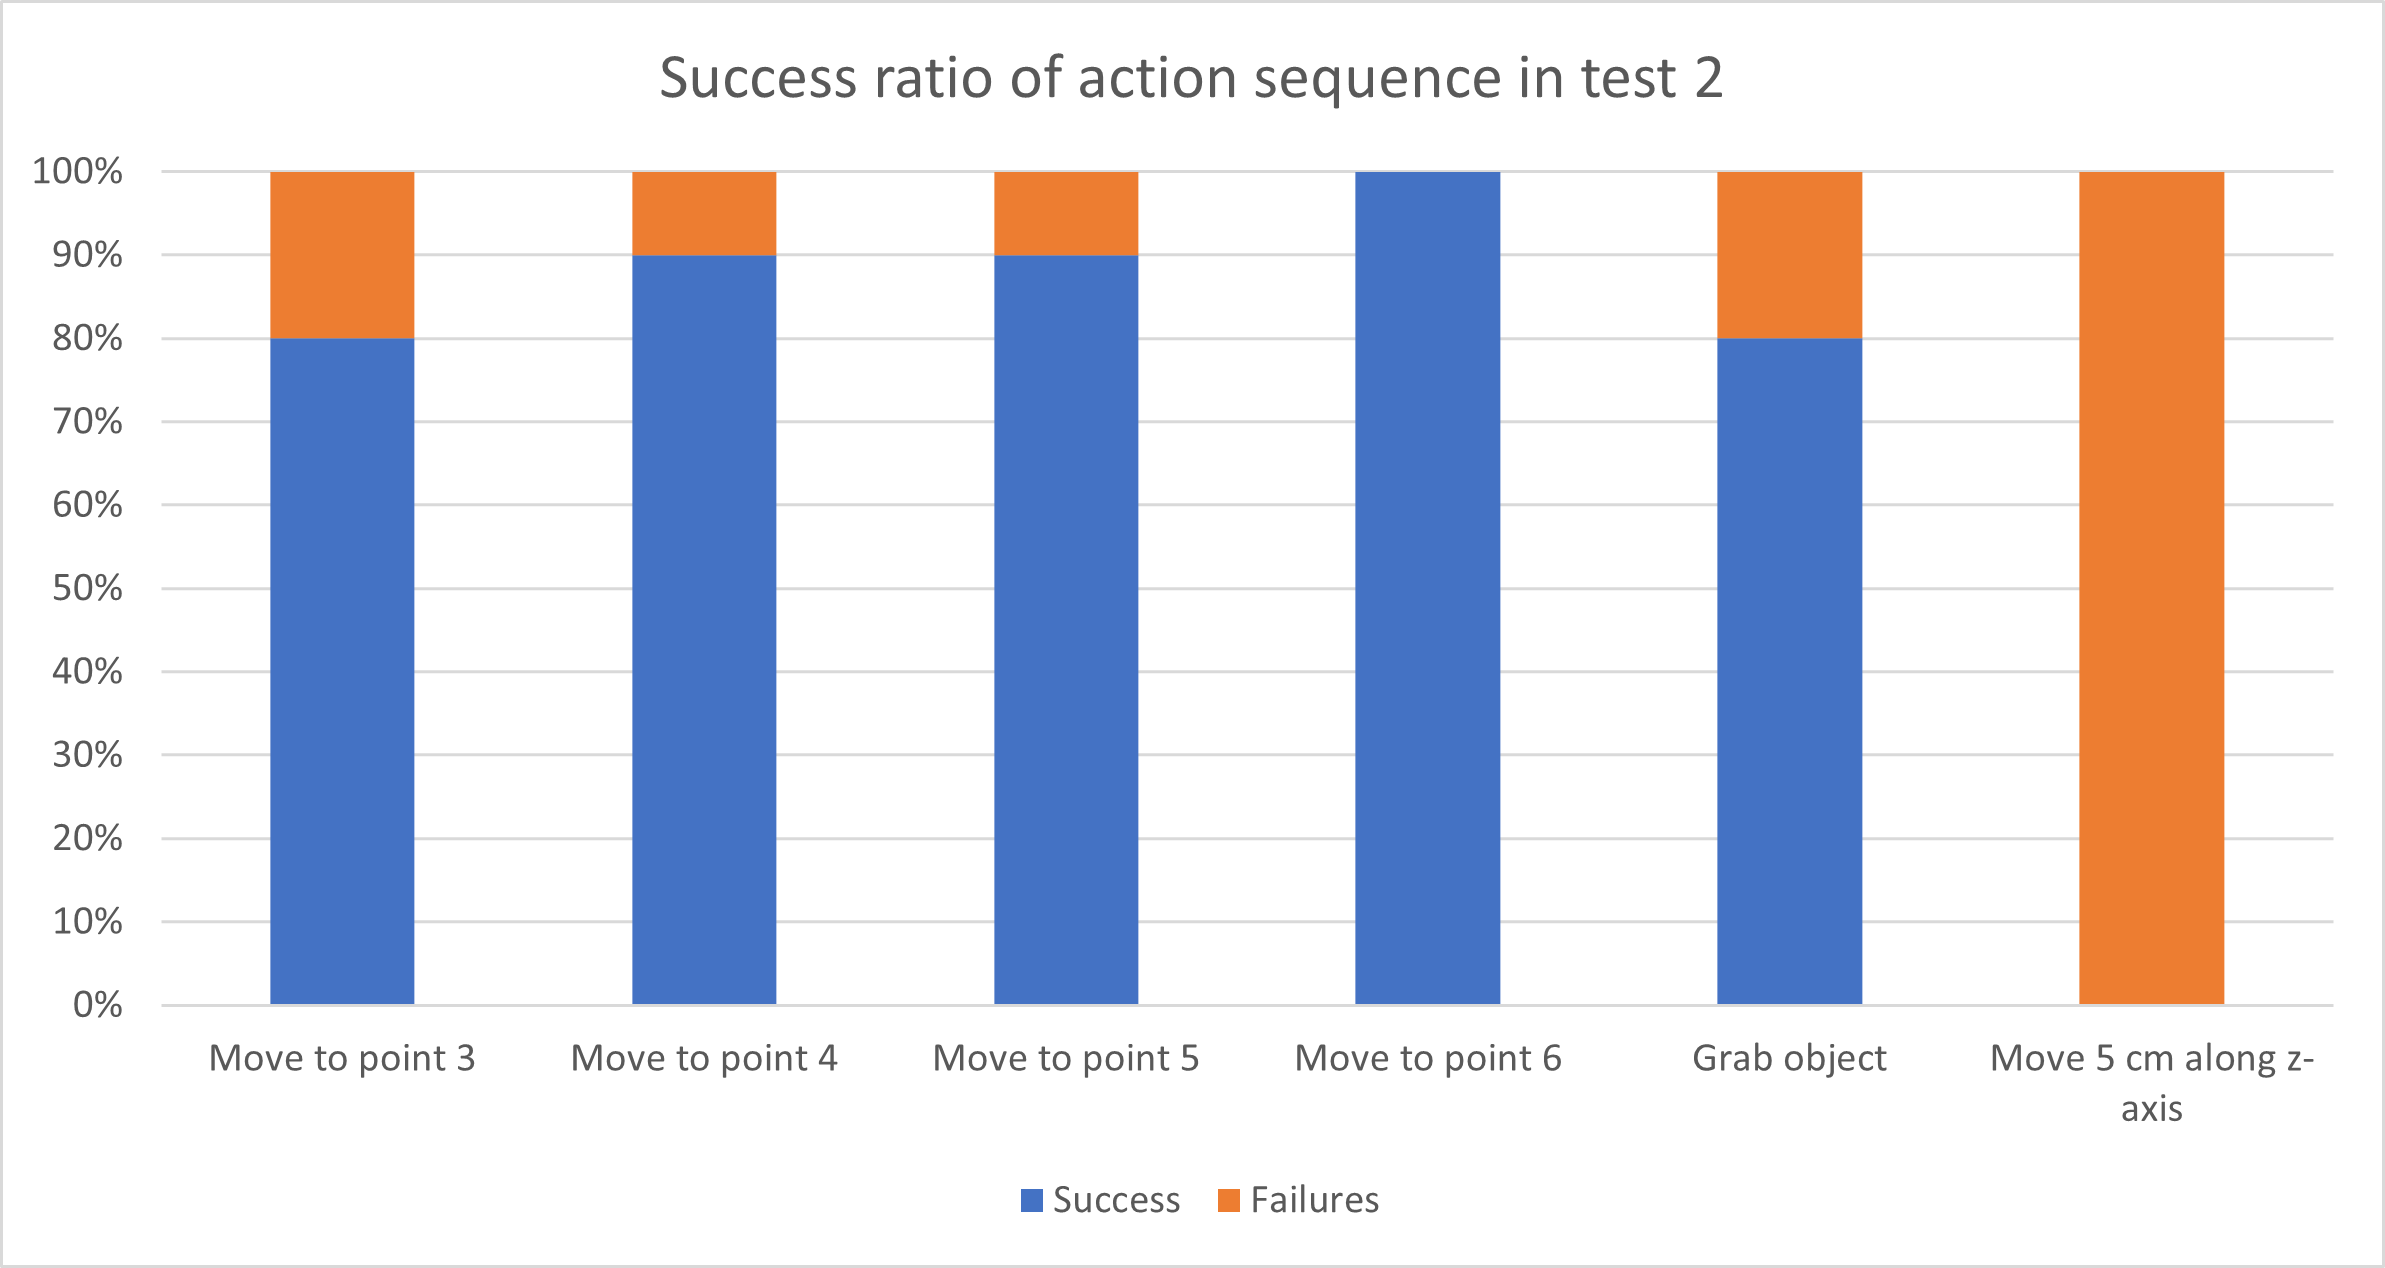
\includegraphics[width=9cm]{img/test_results_2.png}
    \caption{Success ratio of each action in task 2.}
    \label{fig:eval_test_2}
\end{figure}

\begin{figure}[ht]
    \centering
    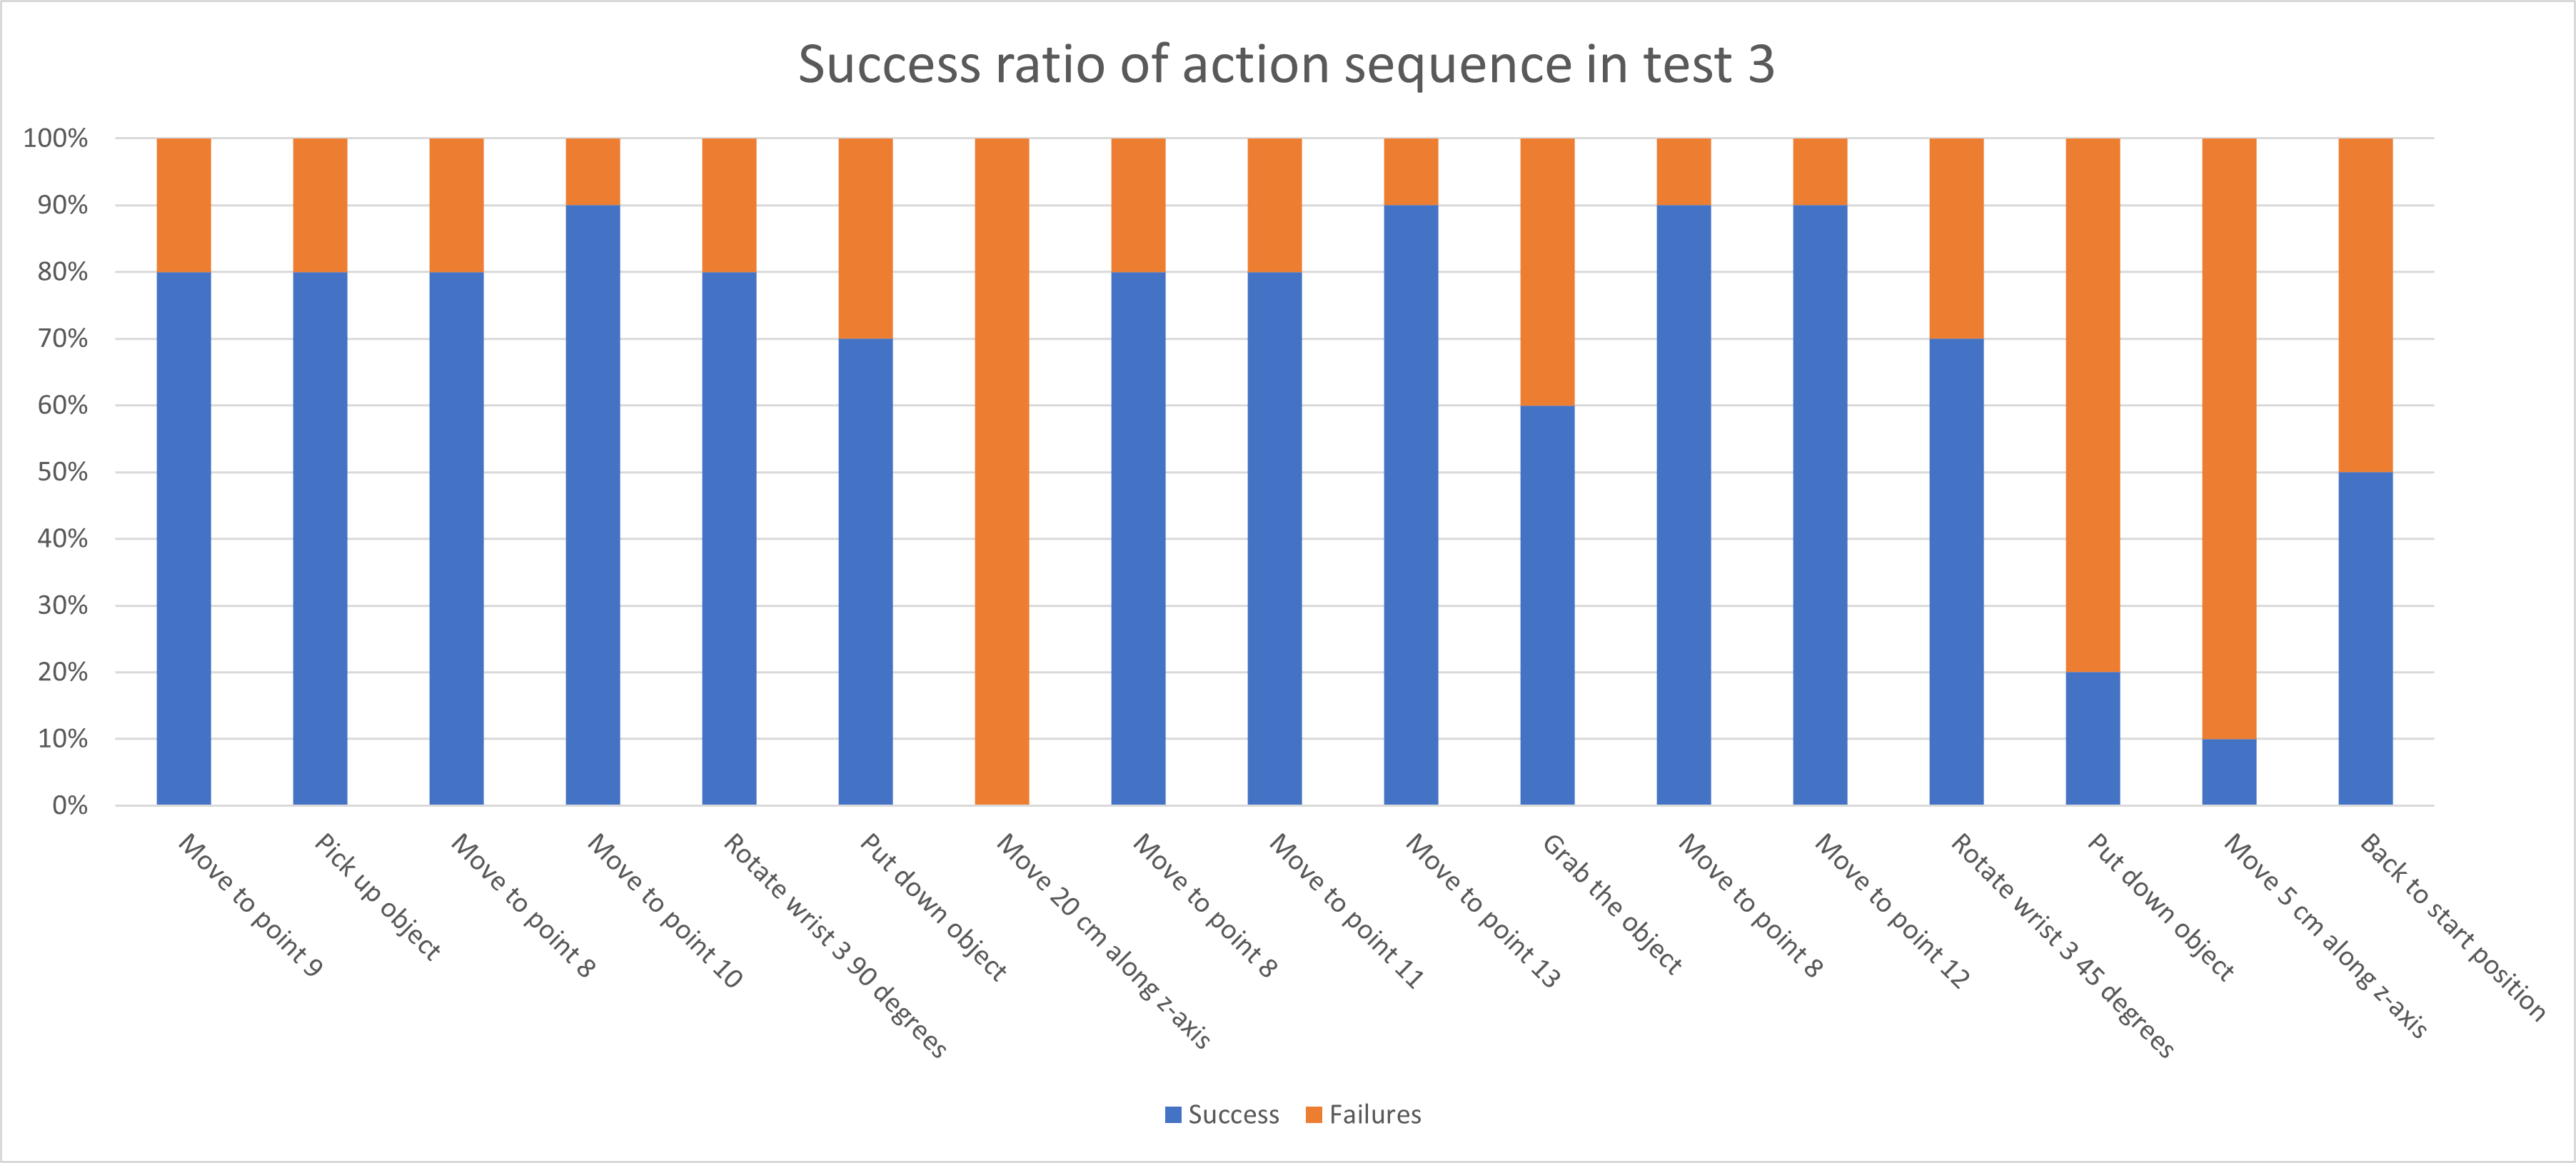
\includegraphics[width=16cm]{img/test_results_3.png}
    \caption{Success ratio of each action in task 3.}
    \label{fig:eval_test_3}
\end{figure}


\begin{figure}[ht]
    \centering
    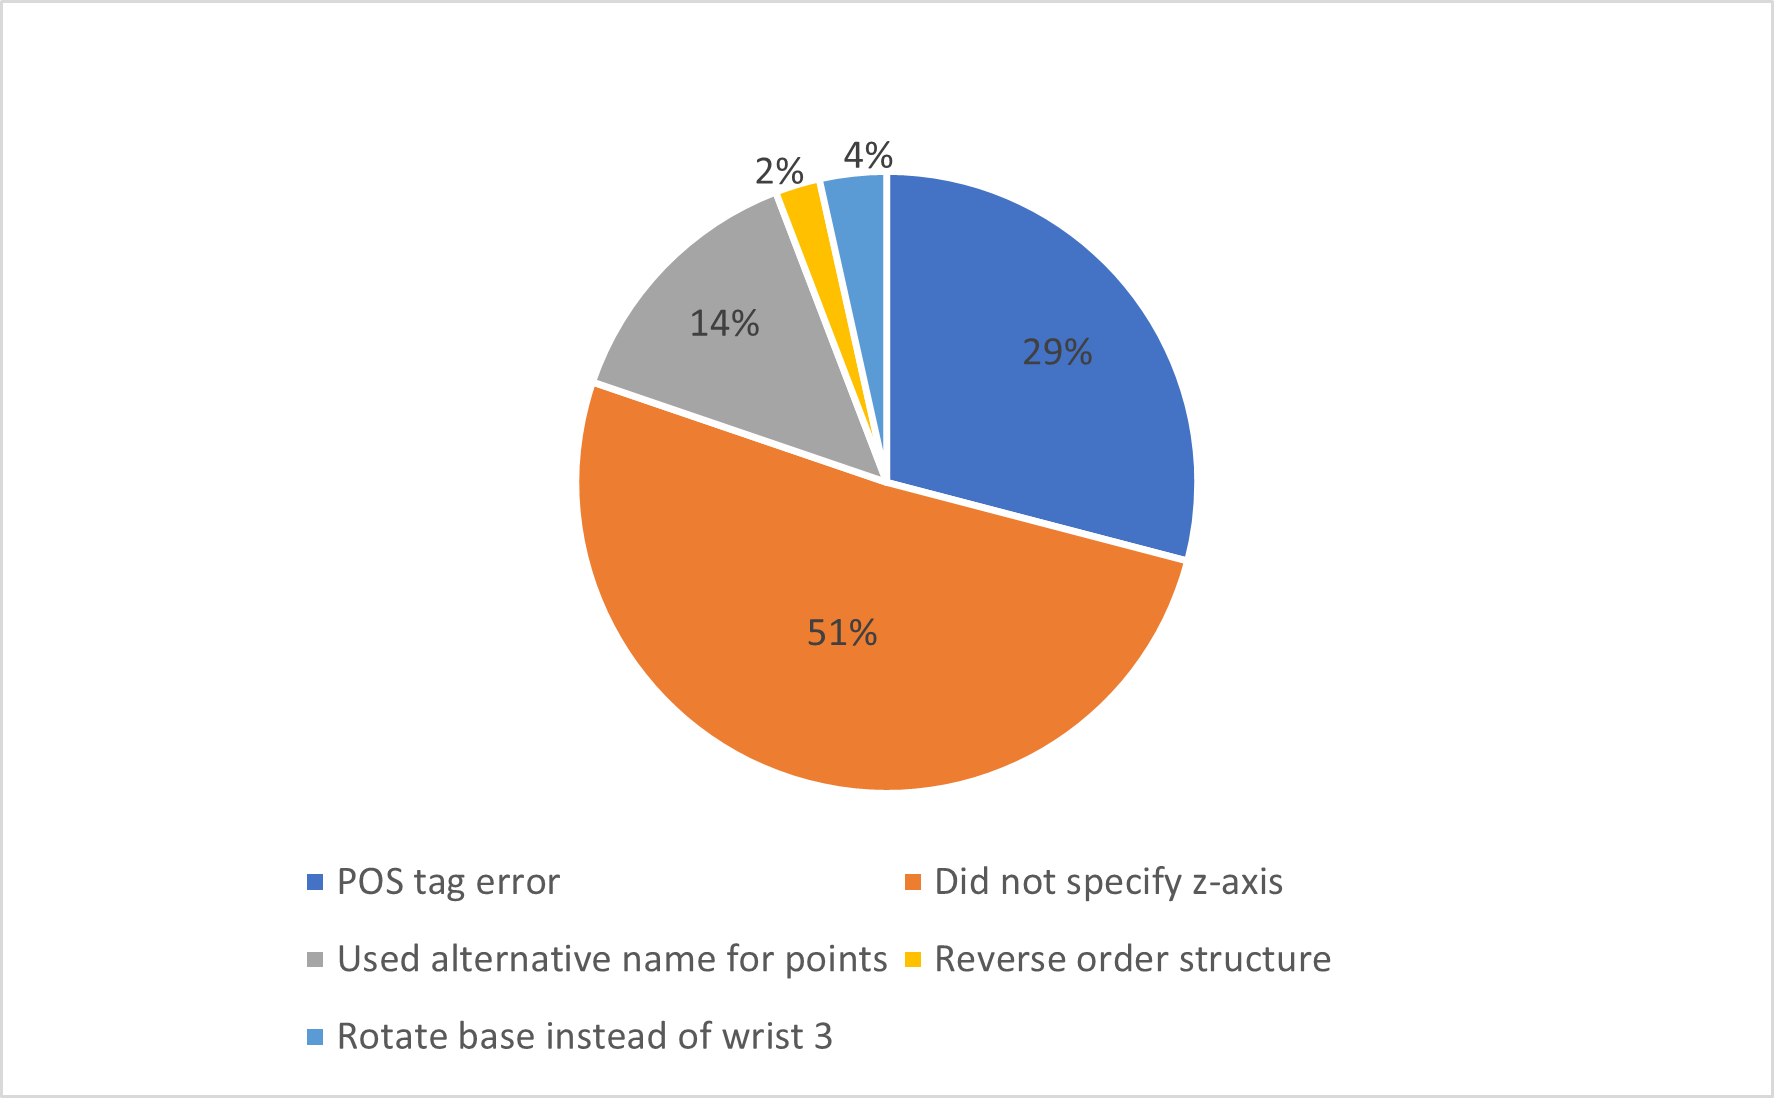
\includegraphics[width=12cm]{img/Error_types.png}
    \caption{Graph showing the type of errors made.}
    \label{fig:error}
\end{figure}


\begin{figure}[ht]
    \centering
    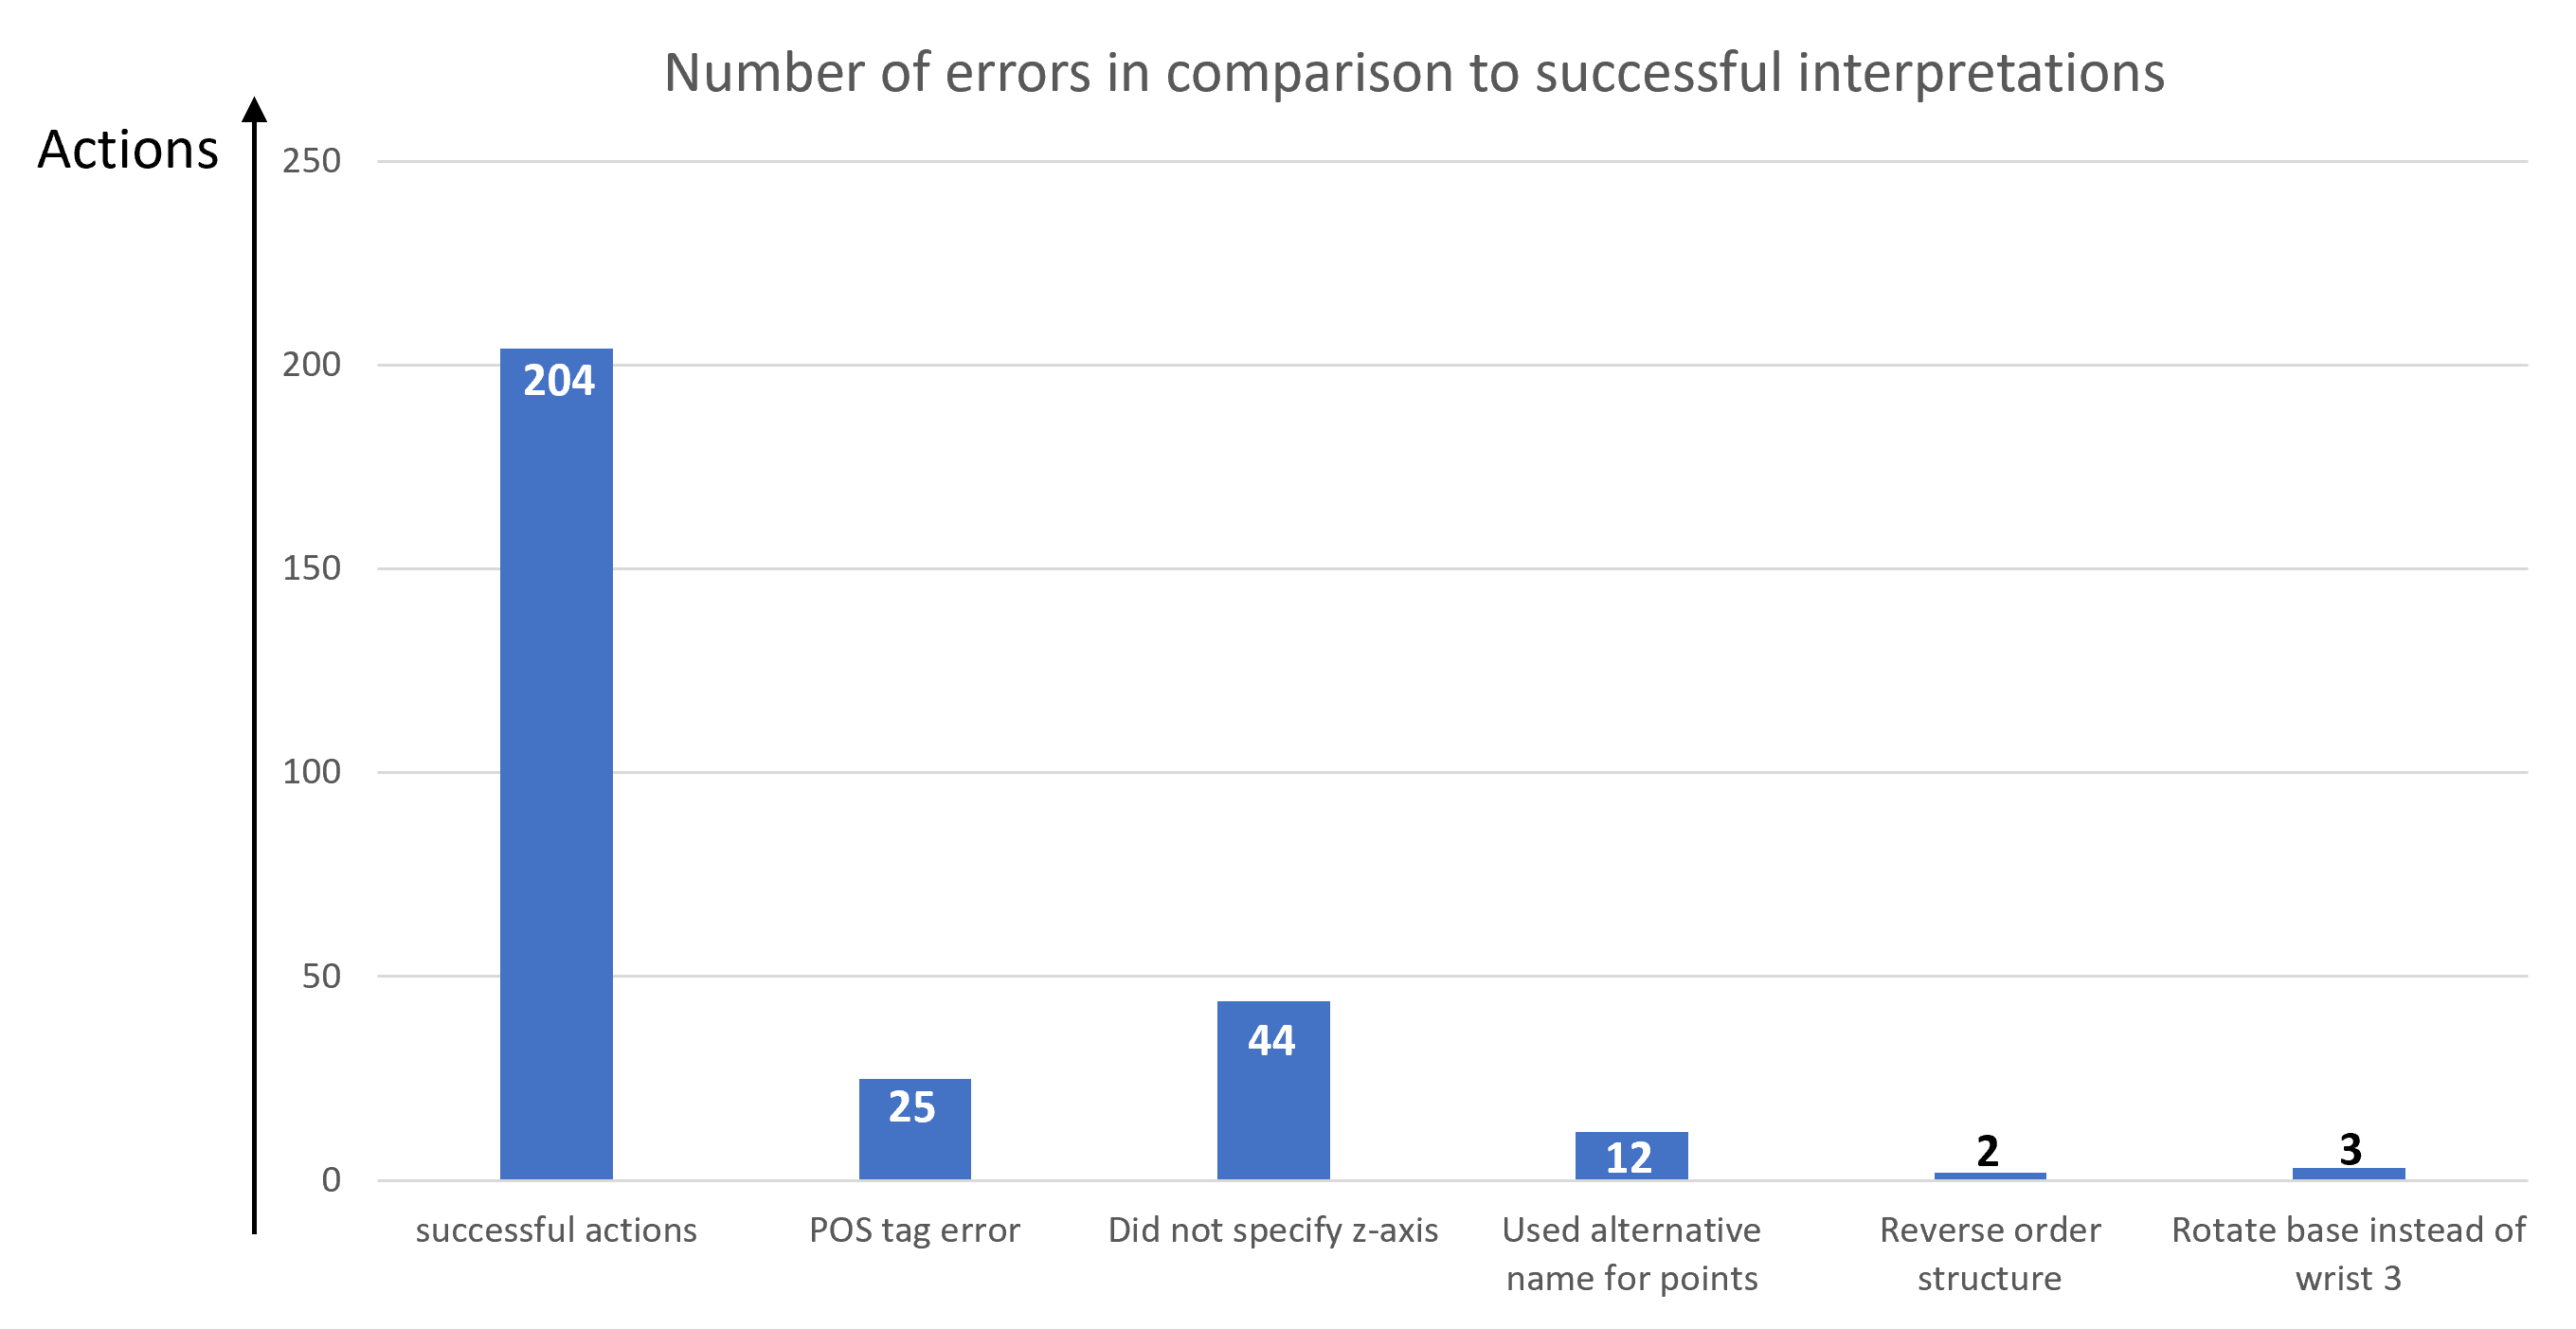
\includegraphics[width=12cm]{img/errors_numerical.png}
    \caption{Graph showing the number of errors made in comparison to successfull interpretations.}
    \label{fig:error_num}
\end{figure}

